\documentclass[a4paper,12pt]{article}

% --- Packages ---
\usepackage[utf8]{inputenc}
\usepackage[T1]{fontenc}
\usepackage{graphicx}
\usepackage{geometry}
\usepackage{hyperref}
\usepackage{booktabs}
\usepackage{float}
\usepackage{setspace}
\usepackage{times}
\geometry{margin=1in}
\onehalfspacing

\begin{document}

%--------------------------------------------------
% COVER PAGE (MACE FORMAT)
%--------------------------------------------------

\begin{titlepage}
\begin{center}

\vspace{1.5cm}

\textbf{\large MAR ATHANASIUS COLLEGE OF ENGINEERING}\\
\vspace{0.2cm}
{\small (Govt. Aided Autonomous Institution, NAAC Accredited With A+ Grade)}

\vspace{2cm}

\includegraphics[width=3cm]{logo.png}

\vspace{2cm}

\textbf{\large MICRO PROJECT REPORT}\\
\vspace{0.3cm}
\textbf{\large ON}

\vspace{0.5cm}

\textbf{\large XcelerType}\\
{\small (Typing Speed Tester)}

\vspace{1.8cm}

\textit{Submitted in partial fulfillment of the requirement for the award of}\\
\textit{Master of Computer Application Degree}

\vspace{1.8cm}

\textbf{Submitted by}

\vspace{0.6cm}

\textbf{JIPHIN GEORGE}\\
Department Of Computer Application\\
(MAC25MCA-2033)

\vspace{2cm}

\textbf{2025-2027}

\vfill

\end{center}
\end{titlepage}

\newpage

\tableofcontents
\newpage

%--------------------------------------------------
\section{Introduction}

XcelerType is a web-based Typing Speed Tester developed using Java and the Spring Boot framework. The system is designed to evaluate and improve the typing speed and accuracy of users in real time.

Traditional typing applications often lack dynamic content and real-time feedback. This project addresses these limitations by providing an interactive interface with character-level validation, dynamic paragraph generation, and detailed performance metrics.

The application is lightweight, does not require a database, and follows an efficient architecture for better performance and scalability.

%--------------------------------------------------
\section{Modules / Functionalities}

\begin{itemize}

\item \textbf{Dynamic Text Generation:} Retrieves random text from an external API to provide unique typing content.

\item \textbf{Real-Time Accuracy Tracking:} Compares each typed character with the original text and highlights correctness instantly.

\item \textbf{Performance Metrics:} Calculates Words Per Minute (WPM), Accuracy, and Perfect Words.

\item \textbf{Keyboard Heatmap:} Tracks keypress frequency and displays user typing behavior visually.

\item \textbf{User Interface Controls:} Allows font scaling and theme adjustments.

\item \textbf{Session Management:} Maintains highest score using in-memory storage.

\end{itemize}

%--------------------------------------------------
\section{Technology Used}

\begin{table}[H]
\centering
\begin{tabular}{ll}
\toprule
\textbf{Category} & \textbf{Technology} \\
\midrule
Programming Language & Java 21 \\
Framework & Spring Boot \\
Frontend & HTML, CSS, Tailwind CSS \\
Scripting & JavaScript \\
Template Engine & Thymeleaf \\
Build Tool & Apache Maven \\
API & DummyJSON Quotes API \\
\bottomrule
\end{tabular}
\caption{Technology Stack}
\end{table}

%--------------------------------------------------
\section{Implementation}

The XcelerType system is implemented using the Model-View-Controller (MVC) architecture, ensuring a clear separation between user interface, business logic, and request handling.

\subsection{Overall Working}

The application follows a structured flow:

\begin{enumerate}
    \item The user accesses the home page through a web browser.
    \item A typing paragraph is dynamically generated using an external API.
    \item The user begins typing, and each keystroke is monitored in real time.
    \item After completion or timeout, the data is sent to the backend.
    \item The backend calculates performance metrics and displays the result.
\end{enumerate}

\subsection{Controller Layer}

The controller is responsible for handling HTTP requests and managing the flow between frontend and backend.

\begin{itemize}
    \item The \texttt{TypingController} class maps URLs such as:
    \begin{itemize}
        \item \texttt{GET /} – Loads the typing interface
        \item \texttt{POST /result} – Processes typing results
    \end{itemize}
    
    \item It retrieves the typing text, collects user input, and sends data to the service layer.
    
    \item After processing, it returns the appropriate view (index or dashboard).
\end{itemize}

\subsection{Service Layer}

The service layer contains the core logic of the application.

\begin{itemize}

    \item \textbf{WPM Calculation:}
    \[
    WPM = \frac{\text{Total Characters Typed} / 5}{\text{Time in Seconds} / 60}
    \]

    \item \textbf{Accuracy Calculation:}
    The system compares typed words with the original words and calculates:
    \[
    Accuracy = \frac{\text{Correct Words}}{\text{Total Words}} \times 100
    \]

    \item \textbf{Highest Score Tracking:}
    The system stores the highest WPM achieved during runtime and updates it if a new score exceeds the previous value.

\end{itemize}

\subsection{Frontend Implementation}

The frontend is developed using HTML, CSS, and JavaScript.

\begin{itemize}
    \item The paragraph is split into individual characters and displayed using \texttt{<span>} elements.
    
    \item JavaScript monitors user input through event listeners:
    \begin{itemize}
        \item \texttt{input event} – Validates each typed character
        \item \texttt{keydown event} – Tracks keypress frequency
    \end{itemize}
    
    \item Based on comparison:
    \begin{itemize}
        \item Correct characters are highlighted in green
        \item Incorrect characters are highlighted in red
    \end{itemize}
\end{itemize}

\subsection{Timer Mechanism}

A timer is implemented using JavaScript:

\begin{itemize}
    \item A countdown of 60 seconds starts when typing begins.
    \item When the timer ends, the test is automatically submitted.
\end{itemize}

\subsection{Heatmap Generation}

The application tracks how many times each key is pressed:

\begin{itemize}
    \item Keypress data is stored in a JavaScript object.
    \item The data is sent to the backend in JSON format.
    \item The dashboard visualizes this data as a keyboard heatmap.
\end{itemize}

\subsection{Data Flow Summary}

\begin{enumerate}
    \item User input is captured in the browser.
    \item Data is sent to the controller via POST request.
    \item The controller passes data to the service layer.
    \item The service processes calculations.
    \item Results are returned and displayed using Thymeleaf.
\end{enumerate}

%--------------------------------------------------
\section{Screenshots with Explanation}

\begin{figure}[H]
\centering
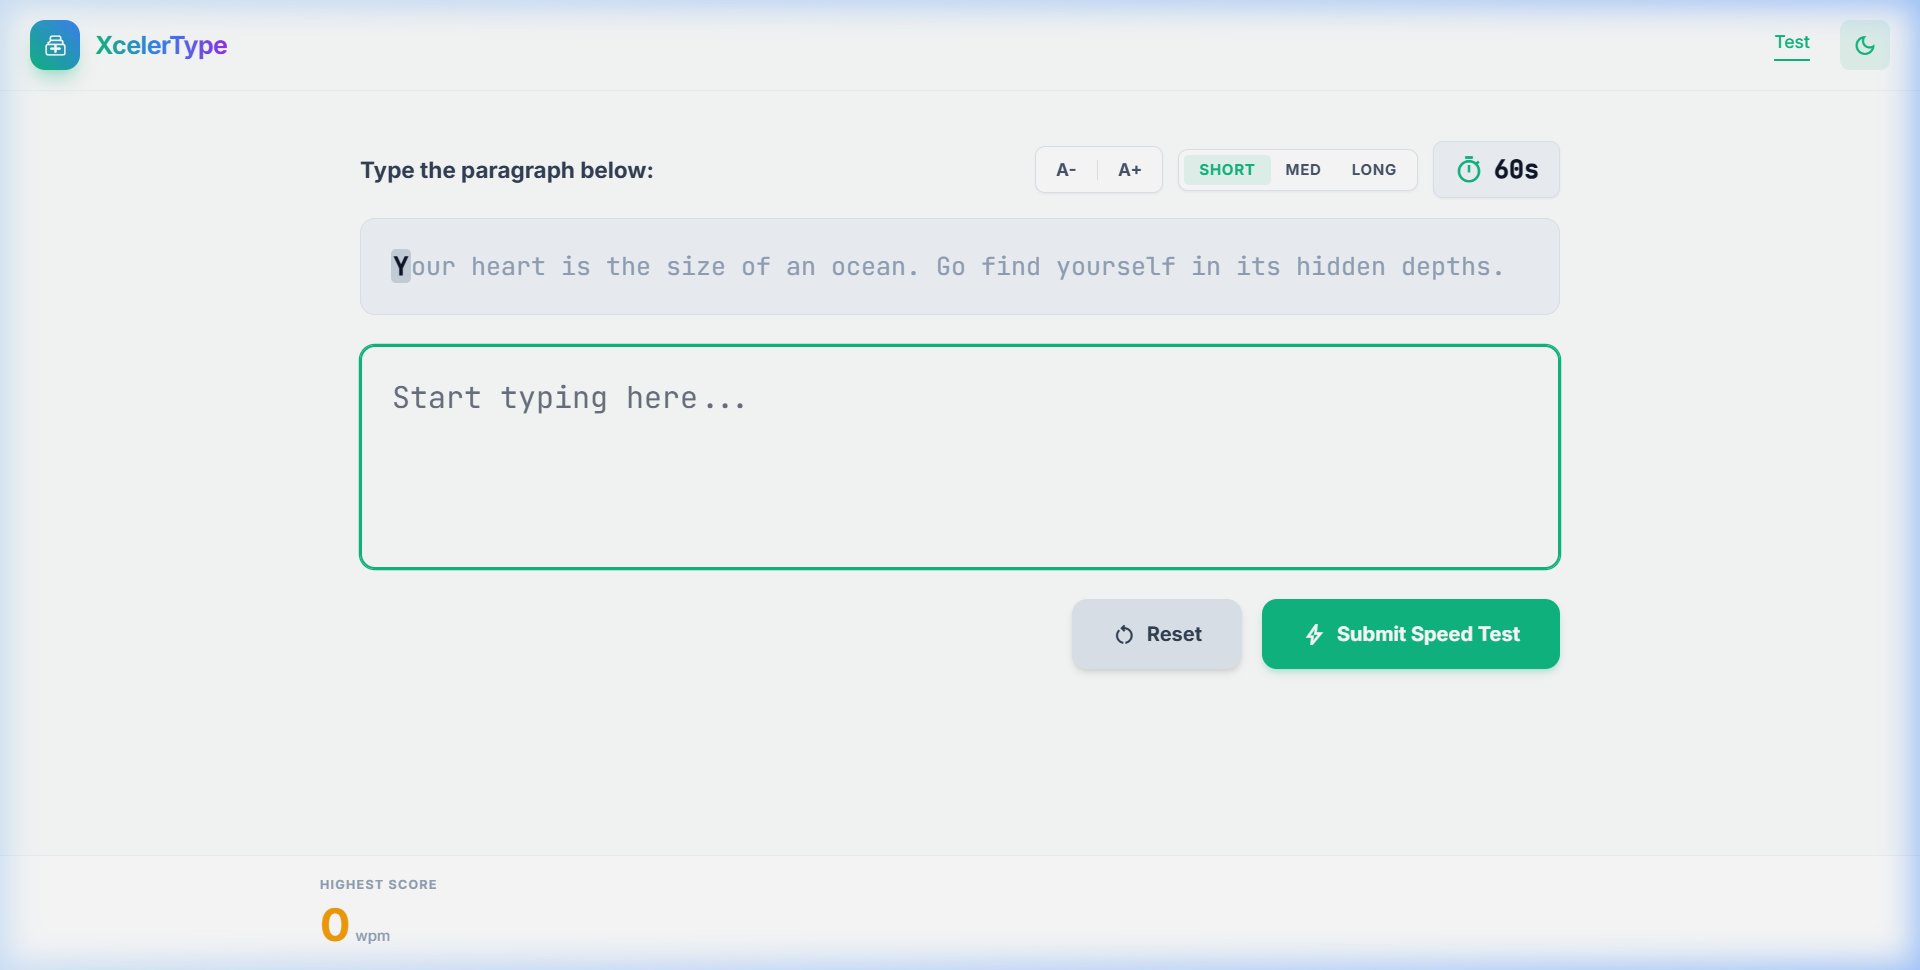
\includegraphics[width=0.85\textwidth]{assets/typing_interface.png}
\caption{Typing Interface showing real-time feedback and timer.}
\end{figure}

\begin{figure}[H]
\centering
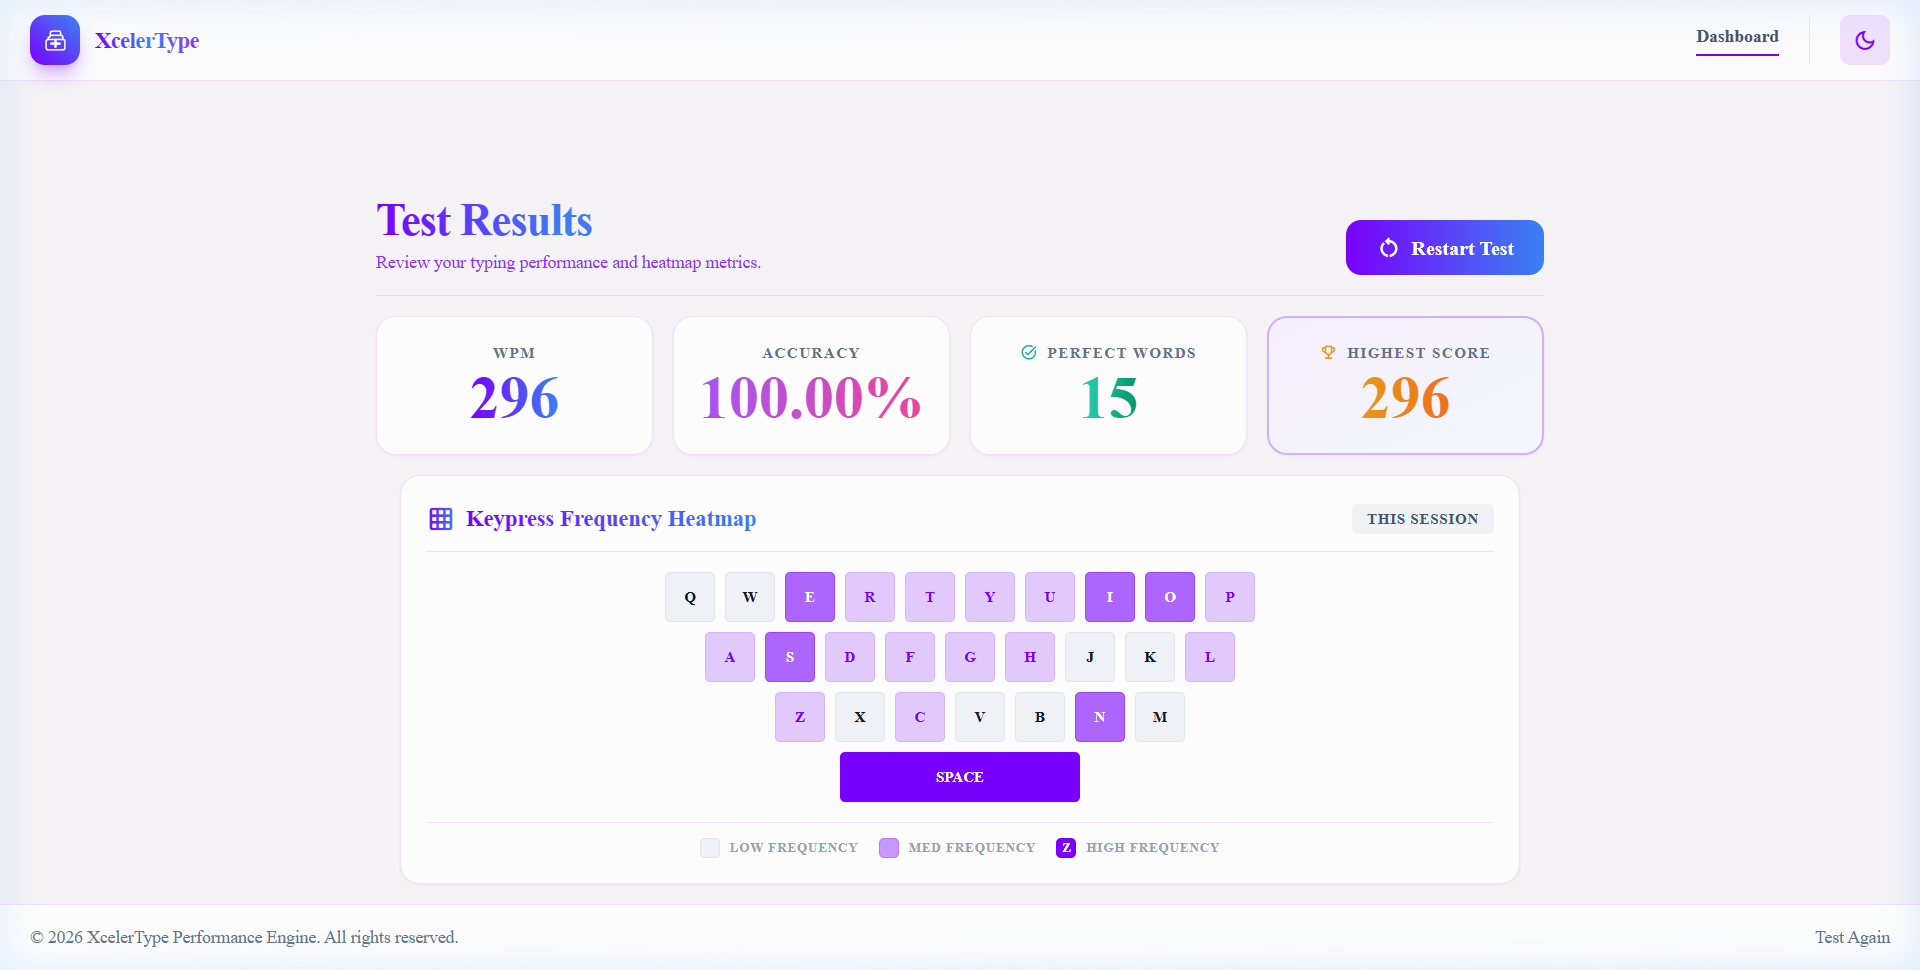
\includegraphics[width=0.85\textwidth]{assets/dashboard_results.png}
\caption{Dashboard displaying WPM, accuracy, and heatmap.}
\end{figure}

%--------------------------------------------------
\section{Conclusion \& References}

\subsection{Conclusion}

The XcelerType application demonstrates an efficient typing evaluation system using modern web technologies. It provides real-time feedback, accurate performance metrics, and a user-friendly interface.

Future enhancements may include database integration, user authentication, and leaderboard features.

\subsection{References}

\begin{itemize}
\item \url{https://spring.io/projects/spring-boot}
\item \url{https://developer.mozilla.org}
\item \url{https://maven.apache.org}
\end{itemize}

\end{document}